\documentclass[runningheads]{llncs}
\pagestyle{plain}
\usepackage[T1]{fontenc}
\usepackage{amsmath,amssymb}
\usepackage{booktabs}
\usepackage{array}
\usepackage{graphicx}
\usepackage[table]{xcolor}
\usepackage{tikz}
\usetikzlibrary{automata,positioning,arrows.meta}
\usepackage{hyperref}
\hypersetup{hidelinks}

\newcommand{\F}{\mathbb{F}}
\newcommand{\DDT}{\mathrm{DDT}}
\newcommand{\LAT}{\mathrm{LAT}}
\newcommand{\BCT}{\mathrm{BCT}}
\newcommand{\Sig}{\Sigma}
\newcommand{\re}[1]{\texttt{#1}}
\newcommand{\wt}{\mathrm{wt}}

\begin{document}

\title{An Automaton-Theoretic Representation of\\ Difference Distribution Tables}
\titlerunning{An Automaton-Theoretic Representation of DDTs}
\author{Anonymous Submission}
\authorrunning{Anonymous Submission}
\institute{}
\maketitle

\begin{abstract}
Differential cryptanalysis, introduced by Biham and Shamir, centers on the
difference distribution table (DDT) of an S-box. For an $n$-bit S-box the table
is a dense $2^{n}\times 2^{n}$ matrix, and even when it fits in memory the
cryptanalytic tasks performed over it are each implemented as an ad-hoc scan,
written anew for every analysis. We argue that the right abstraction for the
DDT is not a matrix but a formal language: by recursively partitioning the table
into quadrants, every cell is identified with a unique word over a quaternary
alphabet $\Sigma = \{\texttt{0},\texttt{1},\texttt{2},\texttt{3}\}$, the non-zero entries form a
regular language $L(D)$, and a quaternary analogue of multi-terminal binary
decision diagram reduction makes the recognizing automaton canonical. The
disparate ad-hoc scans then collapse into a single uniform recipe: any property
definable over $\Sigma$ becomes a query automaton, intersection with $L(D)$ is
standard, and the matching entries are recovered by a joint traversal that
never materializes the matrix. We develop this query calculus, validate seven
query families against exhaustive search, and show that the same construction
and calculus apply verbatim to the linear approximation and boomerang
connectivity tables, unifying differential, linear, and boomerang queries under
a single engine. The representation is also compact: evaluated on the entire
SageMath S-box library, $288$ S-boxes from $n=3$ to $9$ with every automaton
verified cell-by-cell against the dense table, it is competitive with
sparse-bitmap encodings on unstructured S-boxes and improves on them by up to
an order of magnitude on highly structured ones, exactly the cases where
queries are most valuable.
\keywords{Differential cryptanalysis \and Difference distribution table \and
Decision diagrams \and Finite automata \and S-box.}
\end{abstract}

\section{Introduction}

Differential cryptanalysis, introduced by Biham and Shamir~\cite{biham}, is one
of the most influential statistical attacks against symmetric-key primitives. Its
central insight is that the propagation of a chosen input difference through an
iterated cipher is far from uniform, and that pairs of input and output
differences that occur with high probability can be combined into multi-round
trails that distinguish the cipher from a random permutation or recover key
material. In the decades since its introduction, the technique has been refined
into a broad family of variants, including truncated, higher-order, impossible,
and boomerang differential attacks. All of them share the same underlying object:
the difference distribution table of the cipher's nonlinear components, which
records the frequency with which each output difference is produced by each input
difference.

The size of this table is also its main limitation. For an $n$-bit S-box, the DDT
is a $2^{n}\times 2^{n}$ integer matrix, and its exponential growth in $n$ rapidly
exhausts memory budgets. An $8$-bit S-box already requires $64$~KiB; beyond
$n\approx 15$--$16$ the dense matrix can no longer be materialised on commodity
machines. As cryptanalysts increasingly turn their attention to larger S-boxes,
ARX components, and word-oriented permutations, this cost forces a recurring
compromise between the expressiveness of differential analysis and the size of
the primitives that can actually be analysed.

Compounding this storage problem is a more subtle access problem. Even when a DDT
fits in memory, most cryptanalytic tasks do not need every cell at once: they need
to extract the small subset of entries that satisfy some structural property.
Examples are pervasive in the literature, including enumerating all impossible
differentials of an S-box, listing every $(a,b)$ that achieves the differential
uniformity, isolating truncated differentials in which only a few input bits are
active, identifying entries that satisfy a linear relation imposed by the
surrounding cipher, and filtering transitions whose probability lies above a
chosen threshold. In the standard matrix view, each of these queries is solved by
an ad-hoc procedure, written anew for every analysis, and each shares the same
unavoidable lower bound: a full or partial sweep of the table.

In this paper, we argue that the right abstraction for the DDT is not a matrix but
a formal language. By recursively partitioning the table into quadrants, every
cell is identified with a unique word over a quaternary alphabet, and the set of
words that correspond to non-zero entries forms a regular language $L(D)$. This
language is recognised by a finite automaton whose terminal states carry the
differential multiplicities, and whose structure is canonical once a quaternary
analogue of multi-terminal binary decision diagram reduction is applied. The
resulting representation exploits both the general redundancy present in every
DDT, such as the abundance of zero entries, and the specific redundancy resulting
from the algebraic and combinatorial structure of typical S-boxes.

The compactness of this representation is, however, only one half of the
contribution. The other half, and the focus of this work, is the querying
capability that the language-theoretic view unlocks. Once the DDT is encoded as a
regular language, any subset of entries definable by a regular condition over the
alphabet $\Sig=\{0,1,2,3\}$ becomes a regular language in its own right, and can
be intersected with $L(D)$ using standard automata-theoretic constructions. The
disparate ad-hoc scans listed above all collapse into a single uniform recipe:
write the property as a regular expression, compile it into a query automaton,
intersect with the DDT automaton, and enumerate the resulting language. Truncated
differentials, impossible differentials, fixed-bit differentials, entries of
extremal probability, and many other targets that have historically required
specialised code are recovered as one-line queries. Importantly, this also lifts
queries from a per-cell cost to a cost proportional to the size of the (already
compressed) intersection automaton, so the dense matrix never has to be
enumerated even implicitly.

We make three contributions. First, we describe the construction and canonical
reduction of the DDT automaton (Section~\ref{sec:auto}) and evaluate it on the
\emph{entire} SageMath S-box library~\cite{sage}, $288$ S-boxes spanning $n=3$ to
$9$ (Section~\ref{sec:results}); every reported automaton is verified
cell-by-cell against its dense table. Second, we develop the query calculus and
validate seven query families against exhaustive search
(Section~\ref{sec:applications}). Third, we observe that nothing in the
construction is specific to the DDT, and show that the linear approximation table
(LAT) and boomerang connectivity table (BCT) are represented and queried by the
same machinery, placing differential, linear, and boomerang analysis on a common
footing (Section~\ref{sec:beyond}). Section~\ref{sec:conclusion} concludes. A
self-checking artifact reproduces every measurement.\footnote{Artifact anonymised
for review.}

\section{Preliminaries}
\label{sec:prelim}

This section establishes the concepts and notation used throughout, covering the
relevant properties of the cryptanalytic tables, finite automata, and decision
diagrams.

\subsection{Differential cryptanalysis and its tables}

Let $F:\F_2^{n}\to\F_2^{m}$ be a vectorial Boolean function (an S-box). For an
input difference $a$, the derivative of $F$ in direction $a$ is
$D_aF(x)=F(x+a)+F(x)$; counting how often each output difference occurs gives the
difference distribution table.

\begin{definition}[Difference distribution table]
The DDT of $F$ is the $2^{n}\times 2^{m}$ matrix
$\DDT_F[a,b]=\bigl|\{x\in\F_2^{n}:F(x)+F(x+a)=b\}\bigr|$, for $a\in\F_2^{n}$ and
$b\in\F_2^{m}$.
\end{definition}

We assume $m=n$ throughout, as is the case for the permutation S-boxes that
dominate practice, and return to the rectangular case in
Section~\ref{sec:conclusion}. The most studied statistic of the DDT is the
differential uniformity, which upper-bounds an attacker's per-round success
probability and is therefore kept small by design.

\begin{definition}[Differential uniformity]
$\Delta(F)=\max_{a\neq 0,\,b\in\F_2^{m}}\DDT_F[a,b]$.
\end{definition}

\begin{definition}[Differential spectrum]
The differential spectrum of $F$ is the multiset $\{\DDT_F[a,b]:a\neq 0\}$; we
write $\omega_i$ for the number of non-trivial pairs $(a,b)$ with
$\DDT_F[a,b]=i$.
\end{definition}

Zero entries of the DDT are the \emph{impossible differentials}: a transition that
cannot occur immediately discards a key guess reached during partial decryption,
which is the backbone of impossible-differential cryptanalysis. Throughout, the
trivial differential $(0,0)$, whose value is always $2^{n}$, is overridden to $0$;
it carries no cryptanalytic information, and removing it increases the sparsity of
the table.

Two further tables, defined here for use in Section~\ref{sec:beyond}, record the
behaviour of $F$ under the other two main attack families. The linear
approximation table~\cite{matsuilc} $\LAT_F[a,b]=|\{x:a\cdot x=b\cdot
F(x)\}|-2^{n-1}$ collects the correlations of linear approximations, with $\cdot$
the inner product over $\F_2$; its largest off-origin magnitude is the linearity.
For a permutation $F$, the boomerang connectivity table~\cite{bct}
$\BCT_F[a,b]=|\{x:F^{-1}(F(x)+b)+F^{-1}(F(x+a)+b)=a\}|$ makes the boomerang
switch~\cite{wagner} exact, and its boomerang uniformity is
$\beta(F)=\max_{a,b\neq 0}\BCT_F[a,b]$. All three are square integer matrices
indexed by $(a,b)$; they differ only in how a cell is computed.

\subsection{Finite automata and decision diagrams}

A deterministic finite automaton (DFA) over an alphabet $\Sig$ is a tuple
$(Q,\Sig,\delta,q_0,A)$ with transition function $\delta:Q\times\Sig\to Q$,
initial state $q_0$, and accepting set $A$, recognising the regular language
$L=\{w:\delta^{*}(q_0,w)\in A\}$. Regular languages are closed under union,
intersection, and complement; intersection is realised by the product
construction, whose reachable part is what a joint traversal explores.

A binary decision diagram (BDD)~\cite{lee,akers} is a rooted directed acyclic
graph whose internal nodes are labelled by a variable and have two children;
evaluation follows the \texttt{low} or \texttt{high} child according to the bit
read. Bryant~\cite{bryant} showed that fixing a total variable order and applying
two reduction rules---merge isomorphic subgraphs, and delete a node whose children
coincide---yields the reduced ordered BDD, which is canonical and minimal. A
multi-terminal BDD (MTBDD)~\cite{mtbdd} relaxes the terminals from $\{0,1\}$ to an
arbitrary finite set, so that an integer-valued matrix indexed by Boolean
variables is represented by a single canonical diagram. The correspondence between
such diagrams and automata is classical~\cite{kimura}; it is what lets us treat
the diagram as a language recogniser.

\section{An Automaton-Theoretic Representation of DDTs}
\label{sec:auto}

We propose a DDT representation based on automata theory, resting on the
hypothesis that the derivatives of the functions used as S-boxes in real ciphers
are not random, but possess significant structural regularities that can be
exploited for compression. We first identify the redundancy that a dense matrix
fails to exploit, then describe the construction of the automaton and its
reduction.

\subsection{Structural redundancy in DDTs}
\label{sec:redundancy}

For an $n$-bit S-box, representing the DDT as a matrix requires $2^{2n}$ elements,
which quickly becomes prohibitive both for storage and for in-memory analysis as
$n$ grows. The inefficiency of this representation is the result of two kinds of
redundancy. The first is the \emph{general} redundancy present in every DDT:
because the number of distinct differential values is far smaller than the number
of cells, many cells share a value, and at least half of all entries are zero. The
second is the \emph{specific} redundancy induced by the structure of the S-box,
which manifests as the frequent repetition of small identical blocks throughout
the table.

This specific redundancy is already visible in the DDT of the PRESENT S-box, shown
in Table~\ref{tab:present}. Here the table is partitioned into $2\times 2$ blocks
and each block is shaded by how often its pattern occurs, with more frequent
patterns darker. Although the $64$ blocks could in principle realise a great many
distinct patterns, $25$ of them fall into just three patterns---the all-zero
block alone occurs $11$ times---and only $16$ distinct block patterns appear in
total. This repetition is precisely what a quadrant-based encoding can share, and
it is the source of the compression measured in Section~\ref{sec:results}.

\begin{table}[t]
\centering
\caption{The DDT of the PRESENT S-box, partitioned into $2\times2$ blocks and
shaded by pattern frequency (darker $=$ more frequent; zero entries shown as a
dot). Twenty-five of the $64$ blocks fall into the three most common patterns.}
\label{tab:present}
\setlength{\tabcolsep}{0pt}\renewcommand{\arraystretch}{1.1}
\footnotesize
\begin{tabular}{*{16}{@{\hspace{2pt}}c@{\hspace{2pt}}}}
\cellcolor{black!60}. & \cellcolor{black!60}. & \cellcolor{black!36}. & \cellcolor{black!36}. & \cellcolor{black!60}. & \cellcolor{black!60}. & \cellcolor{black!36}. & \cellcolor{black!36}. & \cellcolor{black!36}. & \cellcolor{black!36}. & \cellcolor{black!60}. & \cellcolor{black!60}. & \cellcolor{black!36}. & \cellcolor{black!36}. & \cellcolor{black!60}. & \cellcolor{black!60}.\\[1pt]
\cellcolor{black!60}. & \cellcolor{black!60}. & \cellcolor{black!36}. & \cellcolor{black!36}4 & \cellcolor{black!60}. & \cellcolor{black!60}. & \cellcolor{black!36}. & \cellcolor{black!36}4 & \cellcolor{black!36}. & \cellcolor{black!36}4 & \cellcolor{black!60}. & \cellcolor{black!60}. & \cellcolor{black!36}. & \cellcolor{black!36}4 & \cellcolor{black!60}. & \cellcolor{black!60}.\\[1pt]
\cellcolor{black!24}. & \cellcolor{black!24}. & \cellcolor{black!24}. & \cellcolor{black!24}2 & \cellcolor{black!24}. & \cellcolor{black!24}4 & \cellcolor{black!24}2 & \cellcolor{black!24}. & \cellcolor{black!60}. & \cellcolor{black!60}. & \cellcolor{black!24}2 & \cellcolor{black!24}. & \cellcolor{black!46}2 & \cellcolor{black!46}2 & \cellcolor{black!24}2 & \cellcolor{black!24}.\\[1pt]
\cellcolor{black!24}. & \cellcolor{black!24}2 & \cellcolor{black!24}. & \cellcolor{black!24}2 & \cellcolor{black!24}2 & \cellcolor{black!24}. & \cellcolor{black!24}4 & \cellcolor{black!24}2 & \cellcolor{black!60}. & \cellcolor{black!60}. & \cellcolor{black!24}2 & \cellcolor{black!24}2 & \cellcolor{black!46}. & \cellcolor{black!46}. & \cellcolor{black!24}. & \cellcolor{black!24}.\\[1pt]
\cellcolor{black!24}. & \cellcolor{black!24}. & \cellcolor{black!60}. & \cellcolor{black!60}. & \cellcolor{black!24}. & \cellcolor{black!24}4 & \cellcolor{black!46}2 & \cellcolor{black!46}2 & \cellcolor{black!24}. & \cellcolor{black!24}2 & \cellcolor{black!24}2 & \cellcolor{black!24}. & \cellcolor{black!24}2 & \cellcolor{black!24}. & \cellcolor{black!24}2 & \cellcolor{black!24}.\\[1pt]
\cellcolor{black!24}. & \cellcolor{black!24}2 & \cellcolor{black!60}. & \cellcolor{black!60}. & \cellcolor{black!24}2 & \cellcolor{black!24}. & \cellcolor{black!46}. & \cellcolor{black!46}. & \cellcolor{black!24}. & \cellcolor{black!24}2 & \cellcolor{black!24}2 & \cellcolor{black!24}2 & \cellcolor{black!24}4 & \cellcolor{black!24}2 & \cellcolor{black!24}. & \cellcolor{black!24}.\\[1pt]
\cellcolor{black!36}. & \cellcolor{black!36}. & \cellcolor{black!24}2 & \cellcolor{black!24}. & \cellcolor{black!60}. & \cellcolor{black!60}. & \cellcolor{black!24}2 & \cellcolor{black!24}. & \cellcolor{black!24}2 & \cellcolor{black!24}. & \cellcolor{black!13}. & \cellcolor{black!13}4 & \cellcolor{black!24}2 & \cellcolor{black!24}. & \cellcolor{black!6}. & \cellcolor{black!6}4\\[1pt]
\cellcolor{black!36}. & \cellcolor{black!36}4 & \cellcolor{black!24}2 & \cellcolor{black!24}. & \cellcolor{black!60}. & \cellcolor{black!60}. & \cellcolor{black!24}2 & \cellcolor{black!24}. & \cellcolor{black!24}2 & \cellcolor{black!24}. & \cellcolor{black!13}. & \cellcolor{black!13}. & \cellcolor{black!24}2 & \cellcolor{black!24}. & \cellcolor{black!6}. & \cellcolor{black!6}4\\[1pt]
\cellcolor{black!60}. & \cellcolor{black!60}. & \cellcolor{black!24}. & \cellcolor{black!24}2 & \cellcolor{black!13}. & \cellcolor{black!13}. & \cellcolor{black!24}. & \cellcolor{black!24}2 & \cellcolor{black!24}. & \cellcolor{black!24}2 & \cellcolor{black!13}. & \cellcolor{black!13}4 & \cellcolor{black!24}. & \cellcolor{black!24}2 & \cellcolor{black!6}. & \cellcolor{black!6}4\\[1pt]
\cellcolor{black!60}. & \cellcolor{black!60}. & \cellcolor{black!24}2 & \cellcolor{black!24}. & \cellcolor{black!13}4 & \cellcolor{black!13}. & \cellcolor{black!24}2 & \cellcolor{black!24}. & \cellcolor{black!24}2 & \cellcolor{black!24}. & \cellcolor{black!13}. & \cellcolor{black!13}. & \cellcolor{black!24}2 & \cellcolor{black!24}. & \cellcolor{black!6}4 & \cellcolor{black!6}.\\[1pt]
\cellcolor{black!24}. & \cellcolor{black!24}. & \cellcolor{black!46}2 & \cellcolor{black!46}2 & \cellcolor{black!24}. & \cellcolor{black!24}4 & \cellcolor{black!60}. & \cellcolor{black!60}. & \cellcolor{black!24}2 & \cellcolor{black!24}. & \cellcolor{black!24}2 & \cellcolor{black!24}. & \cellcolor{black!24}. & \cellcolor{black!24}2 & \cellcolor{black!24}2 & \cellcolor{black!24}.\\[1pt]
\cellcolor{black!24}. & \cellcolor{black!24}2 & \cellcolor{black!46}. & \cellcolor{black!46}. & \cellcolor{black!24}2 & \cellcolor{black!24}. & \cellcolor{black!60}. & \cellcolor{black!60}. & \cellcolor{black!24}4 & \cellcolor{black!24}2 & \cellcolor{black!24}2 & \cellcolor{black!24}2 & \cellcolor{black!24}. & \cellcolor{black!24}2 & \cellcolor{black!24}. & \cellcolor{black!24}.\\[1pt]
\cellcolor{black!24}. & \cellcolor{black!24}. & \cellcolor{black!24}2 & \cellcolor{black!24}. & \cellcolor{black!24}. & \cellcolor{black!24}4 & \cellcolor{black!24}. & \cellcolor{black!24}2 & \cellcolor{black!46}2 & \cellcolor{black!46}2 & \cellcolor{black!24}2 & \cellcolor{black!24}. & \cellcolor{black!60}. & \cellcolor{black!60}. & \cellcolor{black!24}2 & \cellcolor{black!24}.\\[1pt]
\cellcolor{black!24}. & \cellcolor{black!24}2 & \cellcolor{black!24}4 & \cellcolor{black!24}2 & \cellcolor{black!24}2 & \cellcolor{black!24}. & \cellcolor{black!24}. & \cellcolor{black!24}2 & \cellcolor{black!46}. & \cellcolor{black!46}. & \cellcolor{black!24}2 & \cellcolor{black!24}2 & \cellcolor{black!60}. & \cellcolor{black!60}. & \cellcolor{black!24}. & \cellcolor{black!24}.\\[1pt]
\cellcolor{black!36}. & \cellcolor{black!36}. & \cellcolor{black!46}2 & \cellcolor{black!46}2 & \cellcolor{black!13}. & \cellcolor{black!13}. & \cellcolor{black!46}2 & \cellcolor{black!46}2 & \cellcolor{black!46}2 & \cellcolor{black!46}2 & \cellcolor{black!60}. & \cellcolor{black!60}. & \cellcolor{black!46}2 & \cellcolor{black!46}2 & \cellcolor{black!6}. & \cellcolor{black!6}.\\[1pt]
\cellcolor{black!36}. & \cellcolor{black!36}4 & \cellcolor{black!46}. & \cellcolor{black!46}. & \cellcolor{black!13}4 & \cellcolor{black!13}. & \cellcolor{black!46}. & \cellcolor{black!46}. & \cellcolor{black!46}. & \cellcolor{black!46}. & \cellcolor{black!60}. & \cellcolor{black!60}. & \cellcolor{black!46}. & \cellcolor{black!46}. & \cellcolor{black!6}4 & \cellcolor{black!6}4
\end{tabular}

\end{table}

\subsection{Constructing a finite automaton from a DDT}

To transform a DDT into a finite automaton we employ an encoding used for
quadtrees and image patterns~\cite{quadtree,patterns}. Let $\Sig=\{0,1,2,3\}$ be a
quaternary alphabet. The whole matrix is assigned the empty word $\varepsilon$; we
then partition the $2^{n}\times 2^{n}$ matrix into four equal quadrants and assign
a distinct symbol of $\Sig$ to each. Applied recursively, a sub-matrix labelled
$w$ has its four quadrants labelled $w0,w1,w2,w3$ for the top-left, top-right,
bottom-left, and bottom-right quadrant, until single cells are reached and receive
words of length $n$. The subset of words mapping to non-zero entries is the
\emph{language of the DDT}, written $L(D)$. Figure~\ref{fig:enc} illustrates the
scheme for an $8\times 8$ table.

The symbol read at each level encodes one bit of the row index $a$ and one of the
column index $b$. Writing the symbol as the pair $(a_i,b_i)$, we set
\begin{equation}\label{eq:enc}
  \sigma = 2a_i + b_i,
\end{equation}
so that the input bit is the high bit and the output bit the low bit of $\sigma$,
and the bits are read in the interleaved order $a_{n-1},b_{n-1},\dots,a_0,b_0$,
most significant pair first. For instance, $a=101_2$ and $b=011_2$ give the bit
pairs $(1,0),(0,1),(1,1)$ and hence the word $\re{213}$. This single convention is
used everywhere below; in particular, an input-active position ($a_i=1$) uses the
symbols $\{2,3\}$ and an output-active position ($b_i=1$) uses $\{1,3\}$.

\begin{figure}[t]
\centering
\resizebox{0.92\textwidth}{!}{%
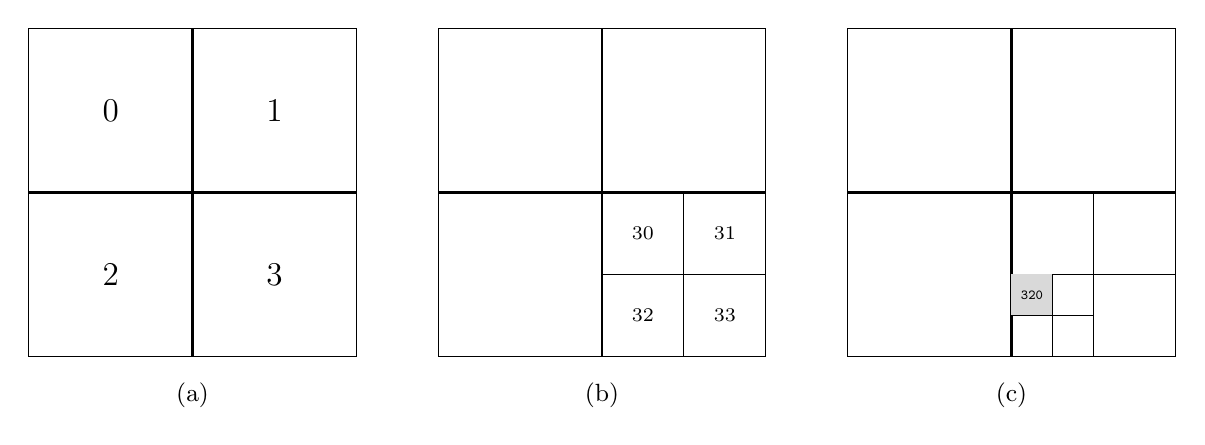
\begin{tikzpicture}[scale=0.52,every node/.style={font=\small}]
 \draw (0,0) rectangle (8,8);
 \draw[thick] (4,0)--(4,8); \draw[thick] (0,4)--(8,4);
 \node at (2,6) {\large 0}; \node at (6,6) {\large 1};
 \node at (2,2) {\large 2}; \node at (6,2) {\large 3};
 \node[below] at (4,-0.4) {(a)};
 \begin{scope}[xshift=10cm]
   \draw (0,0) rectangle (8,8);
   \draw[thick] (4,0)--(4,8); \draw[thick] (0,4)--(8,4);
   \draw (6,0)--(6,4); \draw (4,2)--(8,2);
   \node at (5,3) {\scriptsize 30}; \node at (7,3) {\scriptsize 31};
   \node at (5,1) {\scriptsize 32}; \node at (7,1) {\scriptsize 33};
   \node[below] at (4,-0.4) {(b)};
 \end{scope}
 \begin{scope}[xshift=20cm]
   \draw (0,0) rectangle (8,8);
   \draw[thick] (4,0)--(4,8); \draw[thick] (0,4)--(8,4);
   \draw (6,0)--(6,4); \draw (4,2)--(8,2); \draw (4,1)--(6,1); \draw (5,0)--(5,2);
   \fill[gray!30] (4,1) rectangle (5,2);
   \node at (4.5,1.5) {\tiny\re{320}};
   \node[below] at (4,-0.4) {(c)};
 \end{scope}
\end{tikzpicture}%
}
\caption{Recursive quadrant encoding of an $8\times 8$ DDT. (a) the table split
into four quadrants, each a symbol of $\Sig$; (b) each quadrant split again, so
sub-quadrants receive length-two words; (c) the highlighted cell encoded as
\re{320}.}
\label{fig:enc}
\end{figure}

Following this structural mapping, $L(D)$ is recognised by a quaternary automaton
in which each path from the initial state to a terminal corresponds to a word
$w\in\Sig^{n}$: internal states are the sub-matrices produced by the recursive
partition, and transitions are dictated by the symbols of $\Sig$. Unlike a
standard DFA, which outputs only accept or reject, this automaton must return the
DDT values, so we equip it with a function $f_D:\Sig^{n}\to\mathbb{N}$. Evaluating
a word therefore both decides whether the differential is possible and returns its
multiplicity.

\paragraph{Reduction.}
To store the automaton compactly, minimisation is necessary, but classical DFA
minimisation cannot be applied directly: it would merge accepting states carrying
different values. Instead we draw on the relationship between automata and
decision diagrams~\cite{kimura} and on the integer terminals of the
MTBDD~\cite{mtbdd}, and reduce a quaternary variant of a decision diagram in which
each internal node $v$ has four children $E_0(v),\dots,E_3(v)$:
\begin{enumerate}
  \item terminals are shared, one per distinct value, leaving a single dead
        terminal for $0$;
  \item if $E_0(v)=E_1(v)=E_2(v)=E_3(v)$, node $v$ is redundant and is replaced by
        that common child;
  \item if two internal nodes \emph{at the same level} have identical children,
        they are merged.
\end{enumerate}
The level qualifier in rule~3 reflects that a node's identity in an ordered diagram
is the pair (variable, children): two nodes with the same children at different
depths are distinct, and merging them would corrupt evaluation. While the
resulting automaton is not minimal in the ordinary sense, it is minimal and
canonical in this ordered, multi-terminal setting, by Bryant's
argument~\cite{bryant} transported through the diagram--automaton
correspondence~\cite{kimura}. The final step removes the redundant strings from
the function table, leaving exactly one entry per distinct value.

\paragraph{A worked example.}
To illustrate the construction and its reduction, consider the $3$-bit S-box of
the SEA cipher, whose DDT is shown in Table~\ref{tab:sea}. Because the S-box is
APN, its only non-zero value is $2$, and the trivial differential at $(0,0)$ is
overridden to $0$. The unreduced automaton spells out all $28$ paths to non-zero
cells. Reduction collapses the repeated structure: at the first level the
branches on symbols $0$, $1$, and $2$ lead to identically structured
sub-matrices and are grouped, immediately sparing half the storage, and at the
terminal level a single accepting state suffices for the value $2$. The reduced
automaton, shown in Figure~\ref{fig:sea}, has nine states---eight internal and
accepting states together with the dead terminal---and a function table with the
single entry $2$. We verified that it reproduces all $64$ cells of the DDT
exactly.

\begin{table}[t]
\centering
\caption{DDT of the $3$-bit S-box of the SEA cipher (rows $a$, columns $b$). The
S-box is APN, so every non-zero entry equals $2$.}
\label{tab:sea}
\footnotesize
\begin{tabular}{c|cccccccc}
$a\backslash b$ & 000 & 001 & 010 & 011 & 100 & 101 & 110 & 111\\
\hline
000 & 0 & 0 & 0 & 0 & 0 & 0 & 0 & 0\\
001 & 0 & 2 & 0 & 2 & 0 & 2 & 0 & 2\\
010 & 0 & 2 & 2 & 0 & 0 & 2 & 2 & 0\\
011 & 0 & 0 & 2 & 2 & 0 & 0 & 2 & 2\\
100 & 0 & 0 & 0 & 0 & 2 & 2 & 2 & 2\\
101 & 0 & 2 & 0 & 2 & 2 & 0 & 2 & 0\\
110 & 0 & 2 & 2 & 0 & 2 & 0 & 0 & 2\\
111 & 0 & 0 & 2 & 2 & 2 & 2 & 0 & 0\\
\end{tabular}
\end{table}

\begin{figure}[t]
\centering
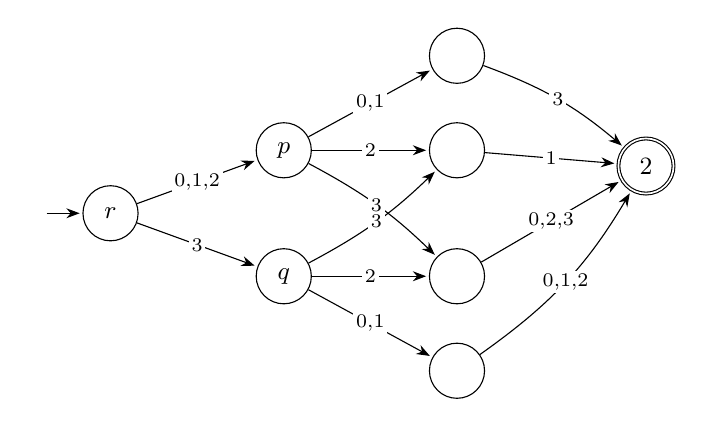
\begin{tikzpicture}[->,>=Stealth,shorten >=1pt,node distance=15mm and 20mm,
   every state/.style={draw,minimum size=7mm,inner sep=1pt,font=\small},on grid]
 \node[state,initial,initial text=] (A) {$r$};
 \node[state] (B) [above right=8mm and 22mm of A] {$p$};
 \node[state] (C) [below right=8mm and 22mm of A] {$q$};
 \node[state] (D) [above right=12mm and 22mm of B] {};
 \node[state] (E) [right=22mm of B] {};
 \node[state] (F) [right=22mm of C] {};
 \node[state] (G) [below right=12mm and 22mm of C] {};
 \node[state,accepting,double] (T) [below right=2mm and 24mm of E] {$2$};
 \tikzset{every node/.style={font=\scriptsize,fill=white,inner sep=1pt}}
 \draw (A) edge node {0,1,2} (B);
 \draw (A) edge node[swap] {3} (C);
 \draw (B) edge node {0,1} (D);
 \draw (B) edge node {2} (E);
 \draw (B) edge[bend left=8] node {3} (F);
 \draw (C) edge[bend right=8] node[swap] {3} (E);
 \draw (C) edge node[swap] {2} (F);
 \draw (C) edge node[swap] {0,1} (G);
 \draw (D) edge[bend left=10] node {3} (T);
 \draw (E) edge node {1} (T);
 \draw (F) edge node[swap] {0,2,3} (T);
 \draw (G) edge[bend right=12] node[swap] {0,1,2} (T);
\end{tikzpicture}
\caption{Reduced automaton for the SEA DDT. Edges are labelled by the symbols
taking each state to its successor; transitions to the dead state are omitted. The
double circle is the single accepting state, of value $2$.}
\label{fig:sea}
\end{figure}

\section{Results}
\label{sec:results}

We evaluated the representation on the SageMath cryptography
library~\cite{sage} (\texttt{sage.crypto.\allowbreak sboxes}), which gathers
$288$ S-boxes from the literature, all square, with widths from $n=3$ to $9$; of
these, $283$ are permutations. For each S-box we built the reduced automaton of
its DDT and verified it cell-by-cell against the dense table computed by Sage,
so every figure below is backed by an exact round-trip. We store the automaton as
a contiguous array of states, each with four fields holding the indices of its
successors; index $0$ is the dead state, accepting states hold the differential
value in place of successors, and the field width follows the state count. We
report the \emph{state ratio}, the dense cell count $2^{2n}$ divided by the number
of automaton states.

\paragraph{Across the library.}
Table~\ref{tab:agg} aggregates the state ratio by S-box size. Compression is
present at every width and increases with $n$, as the larger tables offer more
repeated structure to share. The spread at $n=8$ is wide because the library mixes
strong AES-like S-boxes with deliberately weak or highly structured ones; we
return to the extremes below.

\begin{table}[t]
\centering
\caption{State ratio (dense cells / automaton states) over the SageMath S-box
library, by width, as median~[min--max]. The BCT is restricted to the $283$
permutations.}
\label{tab:agg}
\begin{tabular}{r r c c c}
\toprule
$n$ & \#S-boxes & DDT & LAT & BCT\\
\midrule
3 & 3   & 7.1~[4.9--9.1]    & 3.4~[3.2--5.3]   & 4.0~[3.4--4.9]\\
4 & 215 & 5.2~[4.6--8.8]    & 3.7~[3.1--5.7]   & 3.5~[2.9--9.1]\\
5 & 7   & 10.7~[9.6--11.2]  & 6.5~[6.1--6.6]   & 5.3~[4.8--10.0]\\
6 & 3   & 11.5~[10.7--11.5] & 8.2~[3.9--9.5]   & 11.2~[10.0--11.2]\\
7 & 1   & 10.8              & 4.4              & 8.2\\
8 & 58  & 11.7~[11.5--273.1]& 3.9~[3.4--69.7]  & 10.5~[8.5--125.1]\\
9 & 1   & 217.6             & 75.6             & 27.3\\
\bottomrule
\end{tabular}
\end{table}

\paragraph{Named ciphers.}
Table~\ref{tab:curated} lists a cross-section of well-known S-boxes. The DDT
compression grows with the differential uniformity: a larger $\Delta$ concentrates
the entries into fewer distinct values and larger constant blocks, so the
$\Delta=64$ SKINNY $8$-bit S-box (shared by Romulus, Remus, and ForkSkinny) is
stored in $915$ states ($71.6\times$), and the deliberately weak CSS S-box
($\Delta=128$) in only $240$ states ($273\times$). Translated into memory, the
$64$~KiB AES DDT becomes $42$~KiB, the SKINNY table $7.2$~KiB, and the CSS table
under $1$~KiB; for the $9$-bit DryGASCON S-box the dense $256$~KiB table is stored
in $9.4$~KiB. The byte-level gain is most pronounced exactly when the structural
ratio is, since the field width is otherwise fixed by the state count. The full
per-S-box results for all $288$ S-boxes accompany the artifact.

\begin{table}[t]
\centering
\caption{Reduced DDT automaton for selected S-boxes: state count and state ratio,
with the LAT and BCT ratios of the same S-box (Section~\ref{sec:beyond}).}
\label{tab:curated}
\small
\begin{tabular}{l r r r r r r}
\toprule
S-box & $n$ & $\Delta$ & DDT states & DDT$\times$ & LAT$\times$ & BCT$\times$\\
\midrule
SEA            & 3 & 2   & 9    & 7.1  & 3.4  & 4.0\\
Noekeon        & 4 & 4   & 30   & 8.5  & 4.3  & 7.5\\
PRESENT        & 4 & 4   & 39   & 6.6  & 4.7  & 5.3\\
SKINNY (4-bit) & 4 & 4   & 35   & 7.3  & 3.7  & 5.8\\
PRINCE         & 4 & 4   & 48   & 5.3  & 3.4  & 3.6\\
GIFT           & 4 & 6   & 47   & 5.5  & 4.2  & 3.4\\
Midori $S_{b0}$& 4 & 4   & 52   & 4.9  & 3.5  & 3.6\\
Ascon          & 5 & 8   & 107  & 9.6  & 6.1  & 4.8\\
Fides (5-bit)  & 5 & 2   & 97   & 10.6 & 6.6  & 9.7\\
APN (6-bit)    & 6 & 2   & 356  & 11.5 & 9.5  & 11.2\\
WAGE           & 7 & 8   & 1516 & 10.8 & 4.4  & 8.2\\
AES            & 8 & 4   & 5393 & 12.2 & 3.8  & 12.0\\
Camellia       & 8 & 4   & 5386 & 12.2 & 3.8  & 12.0\\
CLEFIA $S_0$   & 8 & 10  & 5630 & 11.6 & 6.2  & 10.1\\
Skipjack       & 8 & 12  & 5652 & 11.6 & 3.8  & 10.3\\
Kuznyechik     & 8 & 8   & 5590 & 11.7 & 3.8  & 10.6\\
Fantomas       & 8 & 16  & 4556 & 14.4 & 9.1  & 8.5\\
SKINNY (8-bit) & 8 & 64  & 915  & 71.6 & 23.0 & 29.6\\
CSS            & 8 & 128 & 240  & 273.1& 69.7 & 125.1\\
DryGASCON256   & 9 & 128 & 1205 & 217.6& 75.6 & 27.3\\
\bottomrule
\end{tabular}
\end{table}

\section{Applications}
\label{sec:applications}

\subsection{Computing differential properties}

The representation supports the direct computation of standard differential
metrics without ever generating the dense table. The differential uniformity is
the largest value stored at a terminal, found by a single pass over the terminal
set in $O(|T|)$ time, where $|T|\le\Delta(F)+1$. The differential spectrum is
obtained by a depth-first traversal from the root that multiplies the number of
valid transition symbols along each edge and, on reaching a terminal of value
$i$, adds the accumulated path weight to the counter $\omega_i$; this uses $O(n)$
memory and time linear in the number of distinct paths in the reduced structure.
Impossible differentials are exactly the words rejected by the automaton: a
differential $(a,b)$ is impossible iff its encoding is not in $L(D)$. For a single
$(a,b)$ this $O(n)$ evaluation is not advantageous over an $O(1)$ table lookup,
but, as we now show, the language view pays off precisely when many entries are
sought at once under a structural constraint.

\subsection{Complex queries via automata operations}
\label{sec:queries}

Once the DDT is a finite automaton, a cryptanalytic query becomes a regular
\emph{condition} over $\Sig$, resolved by operations on languages. This turns the
ad-hoc search for differential properties into a uniform, language-theoretic
procedure:
\begin{enumerate}
  \item formulate the query as a regular expression $R$ over $\Sig$;
  \item compile $R$ into a finite automaton $Q$;
  \item compute the intersection of $D$ and $Q$ by a joint traversal (a lazy
        depth-first search over the two automata);
  \item enumerate the resulting language, yielding the matching DDT entries.
\end{enumerate}
Because regular languages are closed under union, intersection, and complement,
queries compose: the complement $\overline{L(D)}\cap\Sig^{n}$ is the impossible
language, a value-restricted sub-automaton of $D$ filters by probability, and
products of query automata express conjunctions, all without leaving the
framework. We write $a=a_{n-1}\cdots a_0$ and $b=b_{n-1}\cdots b_0$, use the
encoding~\eqref{eq:enc}, and let \re{.} abbreviate $(0|1|2|3)$.

\begin{description}
\item[Fixed input differences.] To list all possible output differences for a
  fixed input $a=0101$, constrain each position to the corresponding input bit and
  leave the output free, giving $R=\re{(0|1)(2|3)(0|1)(2|3)}$ (positions with
  $a_i=0$ use $\{0,1\}$, those with $a_i=1$ use $\{2,3\}$). This replaces the
  $O(2^{n})$ row scan and is reused for other $a$ by relabelling.
\item[Truncated differentials.] To require only that the two most significant
  input bits be active, $R=\re{(2|3)(2|3)..}$. Any mask in $\{0,1,*\}$ on the
  input and output bits compiles to an automaton of $O(n)$ states; the
  active/inactive special case recovers the activity patterns underlying the
  MILP- and SAT-based active-S-box counts of Mouha et al.~\cite{mouha} and the
  bounds of ciphers such as SKINNY~\cite{skinny}.
\item[Impossible differentials.] These are the words rejected by $D$. Intersecting
  a pattern automaton with $\overline{L(D)}\cap\Sig^{n}$ enumerates the impossible
  cells of that pattern; e.g.\ for a $4$-bit S-box with only the least significant
  input bit active, $R=\re{(0|1)(0|1)(0|1)(2|3)}$. This is the elementary step of
  impossible-differential cryptanalysis as first applied to
  Skipjack~\cite{skipjack} and DEAL~\cite{deal}.
\item[Extremal-probability differentials.] Because each accepting state stores its
  value, filtering by probability is a one-pass restriction of $D$: keep only the
  accepting states with value $\ge\tau$ and prune. Then $L(D_{\ge\tau})$ are the
  differentials of probability $\ge\tau\cdot 2^{-n}$, and $\tau=\Delta(F)$ yields
  those attaining the uniformity, the seed of branch-and-bound trail
  search~\cite{matsui}. The construction visits each accepting state once,
  $O(|S|)$.
\item[Hamming-weight bounded differentials.] The words with $\wt(a)+\wt(b)\le w$
  are accepted by a counter automaton of $O(nw)$ states that adds each symbol's
  popcount ($0$ for \re{0}, $1$ for \re{1} and \re{2}, $2$ for \re{3}).
  Single-bit-in, single-bit-out is
  $R=\re{0*2 0*1 0*}\mid\re{0*1 0*2 0*}\mid\re{0*3 0*}$, supporting the wide-trail
  verification of Daemen and Rijmen~\cite{rijndael}.
\item[Linearly constrained differentials.] The diagonal relation $a=b$ is
  $R=\re{(0|3)}^{n}$, since $\sigma\in\{0,3\}$ exactly when $a_i=b_i$; any
  $\F_2$-linear relation is accepted by a parity-tracking automaton with at most
  $2^{r}$ states for $r$ constraints, extracting the entries compatible with the
  linear context imposed by the surrounding cipher.
\item[Composite and comparative queries.] Boolean closure combines these freely:
  high-probability low-weight differentials are
  $L(D_{\ge\Delta/2})\cap L(\wt\le w)$, a single product. Queries also span two
  S-boxes: given $D_F$ and $D_G$, the language $L(D_F)\setminus L(D_G)$ collects
  the differentials possible for $F$ but impossible for $G$---a certificate of
  inequivalence useful when comparing candidate S-boxes during design.
\end{description}

For every query the running time is dominated by the size of the intersection,
bounded by $|D|\cdot|Q|$ but usually far smaller, and the intersection is never
materialised: a joint traversal touches only the compressed automaton and the
small query automaton, so the memory savings of Section~\ref{sec:results} carry
over to query time.

\subsection{Experimental validation}
\label{sec:query-exp}

The original framework leaves these queries as constructions; we implemented them
and checked each against ground truth. Table~\ref{tab:query} reports, for the
PRESENT ($n=4$) and AES ($n=8$) DDT automata, the number of matching entries and
the number of product states the joint traversal visited, against the $256$ and
$65536$ cells of the dense tables. For every query we also computed the answer by
an exhaustive scan and confirmed set-equality; all seven families agreed exactly.

\begin{table}[t]
\centering
\caption{Validated DDT queries. \emph{res.}\ is the number of matching entries and
\emph{prod.}\ the product states visited; dense tables hold $256$ and $65536$
cells, with $|D|=39$ and $5393$. Every result equals the brute-force set.}
\label{tab:query}
\begin{tabular}{l r r @{\hspace{2.2em}} r r}
\toprule
 & \multicolumn{2}{c}{PRESENT ($n{=}4$)} & \multicolumn{2}{c}{AES ($n{=}8$)}\\
\cmidrule(lr){2-3}\cmidrule(lr){4-5}
query & res. & prod. & res. & prod.\\
\midrule
fixed input difference              & 7  & 18 & 127  & 148 \\
truncated (2 MSB input active)      & 26 & 21 & 8128 & 1405 \\
impossible (one input bit active)   & 12 & 11 & 129  & 135 \\
extremal ($=\Delta$)                & 24 & 40 & 255  & 5395 \\
Hamming $\wt(a)+\wt(b)\le 2$        & 0  & 30 & 24   & 237 \\
linear $a=b$                        & 5  & 17 & 116  & 148 \\
composite ($\ge\Delta/2$, $\wt\le4$)& 63 & 59 & 1091 & 1501 \\
\bottomrule
\end{tabular}
\end{table}

With one exception the traversal visits far fewer product states than the table
has cells. The AES truncated query inspects $1405$ states to enumerate $8128$
matching entries against $65536$ cells, and the structural queries stay in the low
hundreds. The exception is the extremal query, whose value filter is inherently
global and so scans essentially all of $D$ ($5395\approx|S|$), consistent with its
$O(|S|)$ bound and still independent of the dense matrix. The framework also
surfaces structure for free: the empty PRESENT row for $\wt\le 2$ records that the
PRESENT S-box admits no non-trivial differential with at most two active bits.

\section{Beyond the DDT: the LAT and BCT}
\label{sec:beyond}

Nothing in Section~\ref{sec:auto} is specific to the difference distribution
table: the construction takes any square integer matrix over the quadrant
encoding. The linear approximation table and the boomerang connectivity table are
therefore represented by exactly the same reduced automaton, with no change beyond
supplying a different matrix. Their state ratios appear alongside the DDT in
Tables~\ref{tab:agg} and~\ref{tab:curated}. The LAT compresses less than the DDT,
because its values span a range---the AES LAT takes $18$ distinct values against
the DDT's $3$, and the number of terminals bounds the diagram---whereas the BCT,
with a small value set, compresses essentially like the DDT.

The query calculus generalises in the same way, turning linear and boomerang
questions into the same primitive. High-bias linear approximations, which drive
Matsui's attack~\cite{matsuilc}, are the magnitude filter $|\LAT_F[a,b]|\ge\tau$
on the LAT automaton, with $\tau$ the linearity selecting the best approximations.
Boomerang-uniformity cells, the differences that maximise the boomerang
switch~\cite{wagner,bct}, are the value filter $\BCT_F[a,b]=\beta(F)$ on the BCT
automaton. We validated both on the PRESENT and AES tables against an exhaustive
scan (Table~\ref{tab:latbct}); as with the extremal DDT query, these are global
value filters and so scan their table automaton, which is nonetheless far smaller
than---and is built without---the dense matrix. The upshot is that a single
automaton type and a single query engine serve differential, linear, and boomerang
cryptanalysis, with the property of interest residing entirely in the small query
automaton.

\begin{table}[t]
\centering
\caption{Validated LAT and BCT queries against the dense scan; ``lin.''\ is the
linearity and $\beta$ the boomerang uniformity. Product states are reported
against the $256$ (PRESENT) and $65536$ (AES) dense cells.}
\label{tab:latbct}
\begin{tabular}{l l l r r}
\toprule
table & query & S-box & res. & prod.\\
\midrule
LAT & $|\LAT|\ge$ lin. & PRESENT (lin.\ $4$) & 36   & 57\\
LAT & $|\LAT|\ge$ lin. & AES (lin.\ $16$)    & 1275 & 17101\\
BCT & value $=\beta$ & PRESENT ($\beta{=}16$) & 2    & 49\\
BCT & value $=\beta$ & AES ($\beta{=}6$)      & 510  & 5483\\
\bottomrule
\end{tabular}
\end{table}

\section{Conclusion}
\label{sec:conclusion}

We described an automaton-theoretic representation of difference distribution
tables. After outlining the memory and access limitations of the dense matrix, we
reframed the DDT as a formal language and represented it by a reduced quaternary
automaton that captures both the general and the S-box-specific redundancy of the
table. Evaluated on the full SageMath S-box library, the representation reduces
the number of stored states by a median of $5$ to $12\times$, and by up to
$273\times$ for highly structured S-boxes, without any loss of information.

Beyond the storage gain, the central observation is that the language-theoretic
view turns the cryptanalytic searches performed over the table into operations on
automata. The properties that can be phrased as regular conditions over the
quadrant encoding of $(a,b)$---fixed-input and truncated differentials, impossible
differentials, extremal-probability entries, low-weight transitions, linearly
constrained pairs, and composite or cross-table queries---are all recovered
through a single joint traversal of the DDT automaton and a small query automaton,
and we validated each against exhaustive search. Because the construction is
agnostic to how a cell is computed, the same machinery serves the linear
approximation and boomerang connectivity tables, placing the three main attack
families on a common representation.

Several directions extend this work. The square-table assumption can be lifted to
rectangular $2^{n}\times 2^{m}$ tables by an uneven recursion that consumes input
and output bits at different rates. The query class can be enriched from regular to
context-free constraints, such as bounded-difference balances across rounds, by
replacing the query automaton with a pushdown automaton and adapting the joint
traversal. The same automaton can also serve as a generator of linear inequalities
for MILP-based trail search, and quantifying the trade-off between automaton size
and the number of generated inequalities is left to future work. Finally, the size
of the reduced automaton appears to capture an intrinsic notion of the structural
regularity of an S-box, and relating this size-based metric to differential
properties is a natural analytical follow-up.

\begin{thebibliography}{99}
\bibitem{akers} Akers, S.B.: Binary decision diagrams. IEEE Trans. Comput.
  C-27(6), 509--516 (1978)
\bibitem{skinny} Beierle, C., Jean, J., K\"olbl, S., Leander, G., Moradi, A.,
  Peyrin, T., Sasaki, Y., Sasdrich, P., Sim, S.M.: The SKINNY family of block
  ciphers and its low-latency variant MANTIS. In: CRYPTO 2016. LNCS, vol.\ 9815,
  pp.\ 123--153. Springer (2016)
\bibitem{quadtree} Berstel, J., Nait Abdallah, A.: Quadtrees generated by finite
  automata. AFCET 61/62, 167--175 (1989)
\bibitem{patterns} Berstel, J., Morcrette, M.: Compact representation of patterns
  by finite automata. In: PIXIM 89, pp.\ 387--402 (1989)
\bibitem{skipjack} Biham, E., Biryukov, A., Shamir, A.: Cryptanalysis of Skipjack
  reduced to 31 rounds using impossible differentials. In: EUROCRYPT 1999. LNCS,
  vol.\ 1592, pp.\ 12--23. Springer (1999)
\bibitem{biham} Biham, E., Shamir, A.: Differential cryptanalysis of DES-like
  cryptosystems. J. Cryptology 4, 3--72 (1991)
\bibitem{bryant} Bryant, R.E.: Graph-based algorithms for Boolean function
  manipulation. IEEE Trans. Comput. C-35(8), 677--691 (1986)
\bibitem{bct} Cid, C., Huang, T., Peyrin, T., Sasaki, Y., Song, L.: Boomerang
  connectivity table: a new cryptanalysis tool. In: EUROCRYPT 2018. LNCS,
  vol.\ 10821, pp.\ 683--714. Springer (2018)
\bibitem{rijndael} Daemen, J., Rijmen, V.: The Design of Rijndael: AES---The
  Advanced Encryption Standard. Springer (2002)
\bibitem{mtbdd} Fujita, M., McGeer, P.C., Yang, J.C.-Y.: Multi-terminal binary
  decision diagrams: an efficient data structure for matrix representation.
  Formal Methods Syst. Des. 10(2/3), 149--169 (1997)
\bibitem{kimura} Kimura, S., Clarke, E.M.: A parallel algorithm for constructing
  binary decision diagrams. In: ICCD 1990, pp.\ 220--223 (1990)
\bibitem{deal} Knudsen, L.R.: DEAL---a 128-bit block cipher. Technical Report 151,
  University of Bergen (1998)
\bibitem{lee} Lee, C.Y.: Representation of switching circuits by binary-decision
  programs. Bell Syst. Tech. J. 38(4), 985--999 (1959)
\bibitem{matsuilc} Matsui, M.: Linear cryptanalysis method for DES cipher. In:
  EUROCRYPT 1993. LNCS, vol.\ 765, pp.\ 386--397. Springer (1994)
\bibitem{matsui} Matsui, M.: On correlation between the order of S-boxes and the
  strength of DES. In: EUROCRYPT 1994. LNCS, vol.\ 950, pp.\ 366--375. Springer
  (1995)
\bibitem{mouha} Mouha, N., Wang, Q., Gu, D., Preneel, B.: Differential and linear
  cryptanalysis using mixed-integer linear programming. In: Inscrypt 2011. LNCS,
  vol.\ 7537, pp.\ 57--76. Springer (2012)
\bibitem{sage} The Sage Developers: SageMath, the Sage Mathematics Software
  System. \url{https://www.sagemath.org} (module \texttt{sage.crypto.sboxes})
\bibitem{wagner} Wagner, D.: The boomerang attack. In: FSE 1999. LNCS, vol.\ 1636,
  pp.\ 156--170. Springer (1999)
\end{thebibliography}

\end{document}
